\chapter{Probability Spaces and \texorpdfstring{$\sigma$-}{sigma-}algebras}

\section{Prerequisites: Set Theory \& Notation}

Before defining measurable spaces, let us clarify the distinction between a \textbf{set}, a \textbf{collection}, and the notation we use.

\subsection{Set vs. Collection}
\begin{itemize}
    \item \textbf{Sample Space} $\Omega$: The set of all possible outcomes $\omega$.
    \item \textbf{Event} $A$: A subset of $\Omega$ ($A \subseteq \Omega$).
    \item \textbf{Collection} $\mathcal{F}$: A ``set of sets''. It contains events, not outcomes directly.
\end{itemize}

\begin{center}
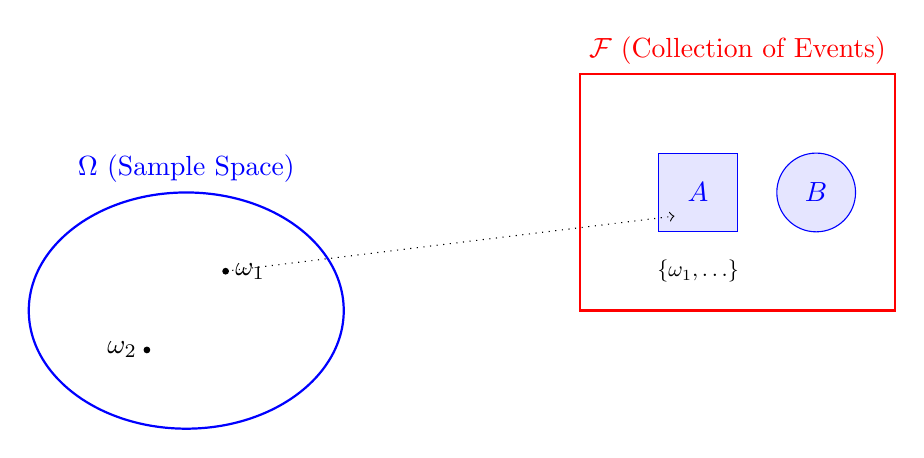
\begin{tikzpicture}
    % Observable Set Omega
    \draw[thick, blue] (0,0) ellipse (2cm and 1.5cm);
    \node[blue] at (0, 1.8) {$\Omega$ (Sample Space)};
    \filldraw[black] (0.5, 0.5) circle (1pt) node[anchor=west] {$\omega_1$};
    \filldraw[black] (-0.5, -0.5) circle (1pt) node[anchor=east] {$\omega_2$};
    
    % Sigma-algebra F
    \draw[thick, red] (5,0) rectangle (9, 3);
    \node[red] at (7, 3.3) {$\mathcal{F}$ (Collection of Events)};
    
    % Subset A inside F
    \draw[blue, fill=blue!10] (6, 1) rectangle (7, 2);
    \node[blue] at (6.5, 1.5) {$A$};
    \node[scale=0.8] at (6.5, 0.5) {$\{ \omega_1, \dots \}$};

    % Subset B inside F
    \draw[blue, fill=blue!10] (8, 1.5) circle (0.5);
    \node[blue] at (8, 1.5) {$B$};
    
    \draw[->, dotted] (0.5, 0.5) -- (6.2, 1.2);
\end{tikzpicture}
\end{center}


\subsection{Example: Two Coin Tosses}
Consider an experiment where we toss a coin twice.
\begin{itemize}
    \item \textbf{Sample Space} $\Omega = \{HH, HT, TH, TT\}$ (4 outcomes).
    \item \textbf{Outcomes}: Simple elements like $\omega_1 = HH$.
    \item \textbf{Events}: Subsets of $\Omega$, e.g., ``Head on first toss'' $A = \{HH, HT\}$.
    \item \textbf{Collection}: A $\sigma$-algebra $\mathcal{F}$ represents solvable questions.
    \begin{itemize}
        \item If we know everything: $\mathcal{F} = 2^\Omega$ (contains $\{HH\}$, $\{HT\}$, etc.).
        \item If we only see the \textbf{first coin}: $\mathcal{F}_1 = \{ \emptyset, \Omega, \{HH, HT\}, \{TH, TT\} \}$.
        \item Note that $\{HH\} \notin \mathcal{F}_1$ because we cannot distinguish $HH$ from $HT$ without seeing the second coin.
    \end{itemize}
\end{itemize}


\subsection{Countable vs. Uncountable}
A set is \textbf{countable} (dénombrable) if you can list its elements in a sequence $x_1, x_2, x_3, \dots$ (potentially infinite).
\begin{itemize}
    \item \textbf{Countable}: Finite sets, $\mathbb{N}$ (integers), $\mathbb{Q}$ (rationals).
    \item \textbf{Uncountable}: $\mathbb{R}$ (reals), $[0, 1]$.
\end{itemize}
This distinction is crucial because $\sigma$-algebras are only closed under \textbf{countable} operations. We cannot sum probabilities over uncountable sets (e.g., $\sum_{x \in [0,1]} P(\{x\})$ makes no sense).

\subsection{Key Notation}
\begin{itemize}
    \item \textbf{Difference} ($A \setminus B$ or $\Omega \setminus A$): "Everything in $\Omega$ except what is in $A$".
    \[ A^c := \Omega \setminus A = \{ \omega \in \Omega : \omega \notin A \} \]
    \item \textbf{Countable Union} ($\bigcup_{n \ge 1} A_n$): The union of a sequence $A_1, A_2, \dots$. It means "at least one of the events $A_n$ occurs".
    \item \textbf{Disjoint Union} ($\bigsqcup$ or "Pairwise Disjoint"): A union where no two sets overlap ($A_i \cap A_j = \emptyset$ for $i \neq j$). This is crucial for adding probabilities: $\mathbb{P}(\bigsqcup A_n) = \sum \mathbb{P}(A_n)$.
    \item \textbf{Power Set} ($2^\Omega$): The set of \textit{all} possible subsets of $\Omega$. If $|\Omega| = n$, then $|2^\Omega| = 2^n$.
\end{itemize}

\section{Measurable Spaces}

The foundation of rigorous probability theory lies in measure theory. Before we can talk about probabilities of events, we must strictly define what an ``event'' is. Not every subset of a sample space can consistently be assigned a probability, especially when dealing with uncountably infinite sample spaces like the real line $\mathbb{R}$.

\begin{definition}[\texorpdfstring{$\sigma$-}{sigma-}algebra]
Let $\Omega$ be a non-empty set (the sample space). A collection $\mathcal{F}$ of subsets of $\Omega$ (i.e., $\mathcal{F} \subseteq 2^{\Omega}$) is called a \textbf{\texorpdfstring{$\sigma$-}{sigma-}algebra} (or \texorpdfstring{$\sigma$-}{sigma-}field) on $\Omega$ if it satisfies the following three axioms:
\begin{enumerate}
    \item \textbf{Empty set}: $\emptyset \in \mathcal{F}$.
    \item \textbf{Complement}: If $A \in \mathcal{F}$, then its complement $A^c := \Omega \setminus A \in \mathcal{F}$.
    \item \textbf{Countable Union}: If $(A_n)_{n \geq 1} \subset \mathcal{F}$ is a sequence of sets in $\mathcal{F}$, then their union is also in $\mathcal{F}$:
    \[
    \bigcup_{n \geq 1} A_n \in \mathcal{F}.
    \]
\end{enumerate}
The pair $(\Omega, \mathcal{F})$ is called a \textbf{measurable space}. The elements of $\mathcal{F}$ are called \textbf{measurable sets} or, in the context of probability, \textbf{events}.
\end{definition}

\begin{remark}
From these axioms, we can deduce other properties:
\begin{itemize}
    \item The whole space $\Omega$ must be in $\mathcal{F}$ because $\Omega = \emptyset^c$.
    \item \textbf{Closed under Countable Operations}: The term "closed" means if you take any countable number of sets from $\mathcal{F}$ and apply set operations (union, intersection, complement), the result stays in $\mathcal{F}$.
    \item \texorpdfstring{$\sigma$-}{sigma-}algebras are closed under countable intersections. By De Morgan's laws:
    \[
    \bigcap_{n \geq 1} A_n = \left( \bigcup_{n \geq 1} A_n^c \right)^c \in \mathcal{F}.
    \]
\end{itemize}
\end{remark}

\subsection{Examples of \texorpdfstring{$\sigma$-}{sigma-}algebras}
\begin{enumerate}
    \item \textbf{Trivial \texorpdfstring{$\sigma$-}{sigma-}algebra}: $\mathcal{F} = \{ \emptyset, \Omega \}$. This is the smallest possible \texorpdfstring{$\sigma$-}{sigma-}algebra. It corresponds to having no information about the outcome of an experiment other than it happened.
    \item \textbf{Power set}: $\mathcal{F} = 2^{\Omega} = \{ A : A \subset \Omega \}$. This is the largest possible \texorpdfstring{$\sigma$-}{sigma-}algebra, containing every possible subset. While useful for discrete spaces (like rolling a die), it is often too large for continuous spaces like $\mathbb{R}$ to define a consistent measure (Vitali sets).
    \item \textbf{Partition-generated}: Let $(A_i)_{i \in I}$ be a countable partition of $\Omega$, meaning $\Omega = \bigsqcup_{i \in I} A_i$ (disjoint union). The \texorpdfstring{$\sigma$-}{sigma-}algebra generated by this partition consists of all possible unions of the sets $A_i$:
    \[
    \mathcal{F} = \left\{ \bigcup_{j \in J} A_j : J \subseteq I \right\}.
    \]
    This structure is very important in finance when modeling information flow in discrete time. If we know which partition element $\omega$ falls into, our information is described by this \texorpdfstring{$\sigma$-}{sigma-}algebra.
\end{enumerate}

\section{Generated \texorpdfstring{$\sigma$-}{sigma-}algebras}

Often provided with a collection of sets of interest, we want to construct the smallest \texorpdfstring{$\sigma$-}{sigma-}algebra that allows us to measure them.

\begin{definition}[Generated \texorpdfstring{$\sigma$-}{sigma-}algebra]
Let $\mathcal{C} \subseteq 2^{\Omega}$ be any collection of subsets of $\Omega$. The \texorpdfstring{$\sigma$-}{sigma-}algebra generated by $\mathcal{C}$, denoted $\sigma(\mathcal{C})$, is the intersection of all \texorpdfstring{$\sigma$-}{sigma-}algebras containing $\mathcal{C}$:
\[
\sigma(\mathcal{C}) := \bigcap_{\mathcal{F} \supset \mathcal{C}, \mathcal{F} \text{ is a } \sigma\text{-algebra}} \mathcal{F}.
\]
It is the \textbf{smallest} \texorpdfstring{$\sigma$-}{sigma-}algebra containing $\mathcal{C}$.
\end{definition}

\subsection{Borel \texorpdfstring{$\sigma$-}{sigma-}algebra}
In topological spaces, we want our algebraic structure (events) to be compatible with the topological structure (open sets, convergence).

\begin{definition}[Borel \texorpdfstring{$\sigma$-}{sigma-}algebra]
Let $(\Omega, \tau)$ be a topological space. The \textbf{Borel \texorpdfstring{$\sigma$-}{sigma-}algebra}, denoted $\mathcal{B}(\Omega)$, is the \texorpdfstring{$\sigma$-}{sigma-}algebra generated by the family of open sets $\mathcal{O}$ in $\Omega$.
\end{definition}

\subsubsection{Case of $\mathbb{R}$ and $\mathbb{R}^d$}
\begin{itemize}
    \item On $\mathbb{R}$, $\mathcal{B}(\mathbb{R})$ is generated by open intervals $]a, b[$. It is the smallest family of sets containing all intervals that is closed under countable operations.
    \item On $\mathbb{R}^d$, $\mathcal{B}(\mathbb{R}^d)$ is generated by open rectangles (or ``hyper-rectangles''):
    \[
    \prod_{i=1}^d ]a_i, b_i[ = \{ \omega = (\omega_1, \dots, \omega_d) \in \mathbb{R}^d : a_i < \omega_i < b_i, \forall i \}.
    \]
\end{itemize}
Note that while $\mathcal{B}(\mathbb{R}^d)$ contains almost any set we can construct explicitly, there do exist \textbf{non-Borel sets}.
    \begin{itemize}
        \item \textbf{Non-Borel Sets}: These are "pathological" sets (like the Vitali set) constructed using the Axiom of Choice. They essentially "break" the concept of length/measure.
        \item We exclude them from our $\sigma$-algebra to ensure mathematical consistency.
    \end{itemize}

    \textbf{Important Note: $\mathcal{B}(\mathbb{R}^d) \neq 2^{\mathbb{R}^d}$}
    \begin{itemize}
        \item The Borel $\sigma$-algebra is strictly smaller than the Power Set.
        \item $\mathcal{B}(\mathbb{R})$ contains only sets constructed from open intervals.
        \item $2^{\mathbb{R}}$ contains \textbf{every} possible subset, including non-measurable ones.
        \item For probability theory, we work with $\mathcal{B}(\mathbb{R})$ to avoid paradoxes.
    \end{itemize}

\subsection{Product \texorpdfstring{$\sigma$-}{sigma-}algebra}
When dealing with multiple random variables or stochastic processes, we work with Cartesian products of spaces.

Let $((\Omega_n, \mathcal{F}_n))_{n \geq 1}$ be a sequence of measurable spaces.
\begin{itemize}
    \item \textbf{Finite Product}: For a finite number of spaces $\Omega_1 \times \dots \times \Omega_n$, the product \texorpdfstring{$\sigma$-}{sigma-}algebra $\mathcal{F}_1 \otimes \dots \otimes \mathcal{F}_n$ is generated by ``rectangles'' of the form:
    \[
    A_1 \times \dots \times A_n, \quad \text{where } A_i \in \mathcal{F}_i.
    \]
    \textbf{Crucial Distinction:}
    \begin{itemize}
        \item $\Omega_1 \times \Omega_2$: Cartesian product of \textbf{points} (the ground space).
        \item $\mathcal{F}_1 \otimes \mathcal{F}_2$: Sigma-algebra generated by rectangles. It is strictly larger than just $\mathcal{F}_1 \times \mathcal{F}_2$ (which is just a set of pairs of sets). The $\otimes$ symbol implies we generate all necessary unions/intersections to make it a valid $\sigma$-algebra.
    \end{itemize}
    Important property: $\mathcal{B}(\mathbb{R}) \otimes \dots \otimes \mathcal{B}(\mathbb{R}) = \mathcal{B}(\mathbb{R}^n)$.
    
    \textbf{Example: Why do we need $\otimes$? (The Circle Problem)}
    Consider the plane $\mathbb{R}^2 = \mathbb{R} \times \mathbb{R}$.
    \begin{itemize}
        \item A "rectangle" is a set $A \times B$ (e.g., $x \in [0,1], y \in [0,1]$).
        \item A Circle $C = \{ (x,y) : x^2 + y^2 \leq 1 \}$ is a valid event we want to measure.
        \item \textbf{Problem}: A circle \textbf{cannot} be written as a single rectangle $A \times B$ or a finite union of them.
        \item \textbf{Solution}: The $\sigma$-algebra $\mathcal{F} \otimes \mathcal{F}$ allows for \textbf{countable unions}. We can approximate the circle with infinitely many small rectangles. Thus, the circle belongs to $\mathcal{F} \otimes \mathcal{F}$, even though it is not a "simple product" of sets.
    \end{itemize}
    
    \item \textbf{Infinite Product}: For the infinite product space $\prod_{n \geq 1} \Omega_n$, the product $\sigma$-algebra $\bigotimes_{n \geq 1} \mathcal{F}_n$ is generated by \textbf{cylinders} with a finite basis. A measurable cylinder is a set of the form:
    \[
    C = \{ \omega \in \prod \Omega_n : \omega_{i_1} \in A_{i_1}, \dots, \omega_{i_k} \in A_{i_k} \}
    \]
    where only a finite number of coordinates are restricted. This is essential because we cannot define a uniform measure on infinite dimensions directly; we must work with these finite-dimensional projections (Kolmogorov Extension Theorem).
\end{itemize}

\section{Probability Measures}

\begin{definition}[Measure]
A map $\mu: \mathcal{F} \to [0, \infty]$ is called a \textbf{measure} if:
\begin{enumerate}
    \item $\mu(\emptyset) = 0$.
    \item \textbf{$\sigma$-additivity}: For any sequence $(A_n)_{n \geq 1} \subset \mathcal{F}$ of \textbf{pairwise disjoint} sets,
    \[
    \mu\left( \bigcup_{n \geq 1} A_n \right) = \sum_{n \geq 1} \mu(A_n).
    \]
\end{enumerate}
\end{definition}

\begin{definition}[Probability Measure]
A measure $\mathbb{P}$ is a \textbf{probability measure} if it satisfies the normalization axiom:
\[
\mathbb{P}(\Omega) = 1.
\]
The triplet $(\Omega, \mathcal{F}, \mathbb{P})$ is called a \textbf{probability space}.
\end{definition}

We denote the set of all probability measures on $(\Omega, \mathcal{F})$ as $\mathcal{P}(\Omega, \mathcal{F})$.

\section{Support of a Measure}

The concept of support formalizes the idea of ``where the probability mass lives''.

\begin{definition}[Support]
The \textbf{support} of a measure $\mu$, denoted $\text{supp}(\mu)$, is the closed set in $\Omega$ such that:
\begin{enumerate}
    \item The measure of its complement is zero: $\mu(\Omega \setminus \text{supp}(\mu)) = 0$.
    \item For any open set $G$ such that $G \cap \text{supp}(\mu) \neq \emptyset$, we have $\mu(G \cap \text{supp}(\mu)) > 0$.
\end{enumerate}
Essentially, it is the smallest closed set that carries all the mass of $\mu$. If measurement values fall outside the support, it is an ``impossible'' event (probability 0).
\end{definition}
For a Polish space (separable, completely metrizable, like $\mathbb{R}^d$), the support is unique and given by:
\[
\text{supp}(\mu) = \Omega \setminus \bigcup \{ V : V \text{ is open and } \mu(V) = 0 \}.
\]
